\section{Описание}

Инструменты, которыми я пользовался: valgrind, plot, perf

Схема директорий:

\begin{itemize}
  \item main.cpp
  \item string.hpp
  \item avltree.hpp
  \item tests\_creator.py
  \item makefile
  \item bash\_script.sh
  \item gnuplot\_script.txt
  \item perf.data
  \item plots (папка с графиками)
  \item tests (папка с тестами)
  \item scrins (папка с скриншотами)
  \item report (папка с отчетом)
\end{itemize}

Во-первых, для того, чтобы анализировать свою программу, время ее исполения и утечки памяти, нужно было написать генератор тестов.
Для данной задачи я выбрал язык Python.

\begin{lstlisting}[language=python]
import random
import copy
from random import choice
from string import ascii_uppercase

randstring = lambda x=1: ''.join(choice(ascii_uppercase) for i in range(x))

if __name__ == "__main__":

    count_of_tests = 5
    max_count_of_commands = 50
    count_of_commands = 1

    actions = ["+", "!", "?", "!"] # + - ? !
    for test_number in range(1, count_of_tests+1):
        tree_elems = {}
        saved = 0
        saved_file = {}
        test_file = open("tests/" + str(test_number) + ".t", 'w')
        file_with_answers = open("tests/" + str(test_number) + ".txt", "w")

        for _ in range( count_of_commands ):
            action = random.choice( actions )
            if action == "+":
                key = randstring()
                value = random.randint( 1, 2**64-1 )
                test_file.write("+ " + key + " " + str(value) + "\n")

                key = key.lower()
                answer = "Exist"
                if key not in tree_elems:
                    answer = "OK"
                    tree_elems[key] = value
                file_with_answers.write(answer + "\n")

            elif action == "-":
                key = randstring()
                test_file.write("- " + key + "\n")

                key = key.lower()
                answer = "NoSuchWord"
                if key in tree_elems:
                    del tree_elems[key]
                    answer = "OK"
                file_with_answers.write(answer + "\n")

            elif action == "?":
                search_exist_element = random.choice( [ True, False ] )
                key = random.choice([key for key in tree_elems.keys()]) if search_exist_element and len(tree_elems.keys()) > 0 else randstring()
                test_file.write(key + "\n")

                key = key.lower()
                if key in tree_elems:
                    answer = "OK: " + str(tree_elems[key])
                else:
                    answer = "NoSuchWord"
                file_with_answers.write(answer + "\n") 
            
            elif action == "!":
                act_file = random.choice(["Load test", "Save test"])
                if act_file == "Save test":
                    test_file.write(action + " " + act_file + "\n")
                    saved_file = tree_elems.copy()
                    file_with_answers.write("OK" + "\n")
                    saved = 1

                elif saved == 1 and act_file == "Load test":
                    test_file.write(action + " " + act_file + "\n")
                    tree_elems = {}
                    tree_elems = saved_file.copy()
                    file_with_answers.write("OK" + "\n")

        count_of_commands+=(max_count_of_commands-count_of_commands)/count_of_tests
\end{lstlisting}

Генератор тестов хорошо работает и не учитывает только случаи, когда нельзя будет открыть файл по каким-то причинам. Поэтому он не сможет проверить ошибки с ERROR.
Так как я хочу испытывать произвольное число тестов и причем их большое количество, я написал bash файл, где будет запускаться моя прорамма, перенаправляя вывод в файл, а
потом с помощью утилиты diff сравнивать файлы от питона и от моей программы.

\begin{lstlisting}[language=bash]
#!/bin/bash
max=6

for ((i = 1; i < ${max}; i++)) 
do 
	echo "test: $i ";
	./main.out < tests/${i}.t > tests/${i}ans.txt;
	echo "ans: $i "; 
	diff tests/${i}ans.txt tests/${i}.txt
done
\end{lstlisting}

Переменная max равняется количеству тестов, которые нужно прогнать.

В самой программе я установил таймер из библиотеки <chrono>, а так же счетчик команд. Результат времени работы программы и счетчик команд выводятся через пробел
в файл time\_log.txt, откуда gnuplot считывает данные и строит график зависимости время исполнения программы от количества входных данных. Для gnuplot так же написан 
скрипт. Мы устанавливаем название осей, расширение изображения, и директорию, куда будет выводиться картинка.

\begin{lstlisting}
set xlabel "data count"
set ylabel "time of appending"
set terminal png
set output "plots/plot.png"
plot "time_log.txt" with lines
pause -1
\end{lstlisting}

Makefile собирает все скрипты вместе и запускает их.

\begin{lstlisting}
#!/bin/bash
CC = g++
FLAGS = -pedantic -Wall -std=c++11 -Werror -Wno-sign-compare -O2 -lm

all: main.out

main.out: main.cpp avltree.hpp string.hpp
	${CC} ${FLAGS} main.cpp -o main.out

run:
	rm -rf time_log.txt
	python tests_creator.py
	./bash_script.sh
	gnuplot gnuplot_script.txt

testss:
	python tests_creator.py
\end{lstlisting}

Первые результаты бенчмарка я опробовал на тестах с только вставкой и на тестах с вставкой, удалением и поиском. 

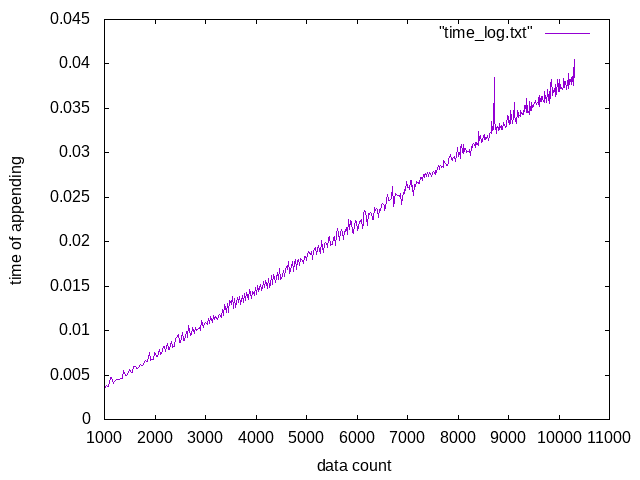
\includegraphics[scale=0.5]{plot1+}
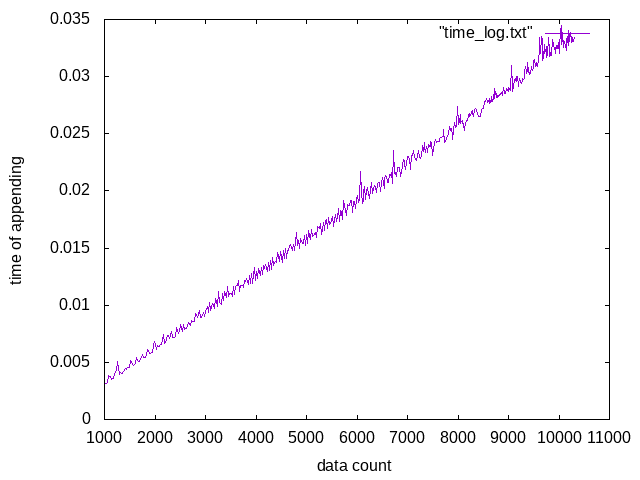
\includegraphics[scale=0.5]{plot2+-?}

Для меня было удивлением увидеть такие результаты, ведь я ожидал график с ассимптотикой $nlog_2 n$, а увидел прямопропорциональную зависимость времени исполения прораммы
от количеств элементов. Поэтому я решил провести тест, где строился график зависимости времени вставки в дерево от количества уже вставленных элементов в него, т.е. время
вставки последнего элемента в дерево.

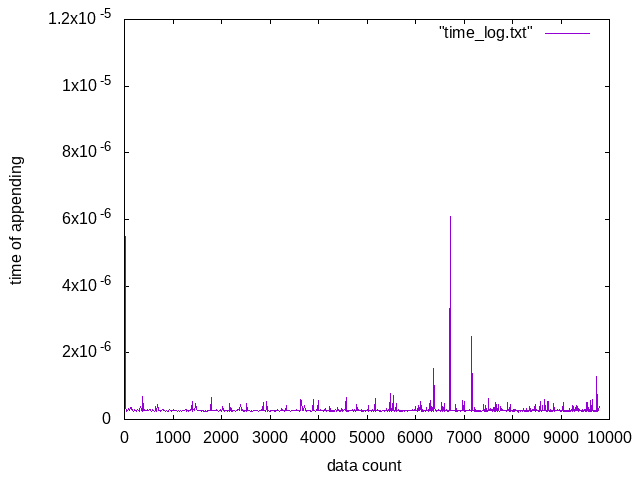
\includegraphics[scale=0.5]{plot6+speedappend} 

И по данному графику я понял, почему два до этого давали такой результат. На таком маленьком числе элементов (порядка 10000) время вставки было практически константным. 
Скорее всего, если бы я мог задействовать одно ядро компьютера полностью под свою программу и взять тесты побольше, то я бы увидел плавный рост, однако не обладая такими
возможностями, я удовлетворился этими результатами.

Несмотря на такие хорошие показатели, моя программа не сразу прошла на чекере и причина тому теперь как никогда ясна - команды Save и Load сильно тормозили процесс. Поэтому
пришло время провести тест, добавив эти две команды. Сначала я использовал версию программы, где загрузка дерева проходила с помощью вставки в обычное бинарное дерево. Потом
я сделал еще одну версию, где сохранение не сильно отличалось от старой, а загрузка производилось с помощью флагов, которые означали есть ли ребенок слева и справа.

\begin{lstlisting}[language=C]
void TAVLTree::Save(const TAVLTree *head, FILE *s) {
  if (head) {
	 	fprintf(s, "%s %llu ", head->key.str, head->value);
	 	Save(head->left, s);
	  Save(head->right, s);
	}
}

TAVLTree* TAVLTree::BinInsert(TAVLTree *head, const NMystd::TString& key, const unsigned long long value) {
	if (head) {
		if (key > head->key) {
			head->right = BinInsert(head->right, key, value);
		} else {
			head->left = BinInsert(head->left, key, value);
		} 
		return head;
	}
	return new TAVLTree(key, value);
}

TAVLTree* TAVLTree::Load(std::ifstream &in) {
	 TAVLTree *res = 0; 
	 char str[256];
	 unsigned long long val;
	 while (fscanf(s, "%s %llu ", str, &val)>0) {
	 	res = res->BinInsert(res, NMystd::TString(str), val);
	 }
	 return res;
}
\end{lstlisting}
\begin{lstlisting}[language=C]
void TAVLTree::Save(const TAVLTree *head, FILE *s) {
	if (!head) {
		return;
	}

	fprintf(s, "%s %llu %u ", head->key.str, head->value, head->h);
	if (head->left) {
		fprintf(s, "1 ");
		Save(head->left, s);
	} else {
		fprintf(s, "0 ");
	}
	if (head->right) {
		fprintf(s, "1 ");
		Save(head->right, s);
	} else {
		fprintf(s, "0 ");
	}
}

TAVLTree* TAVLTree::Load(std::ifstream &in) {
	TAVLTree *res;
	int flag;
	char str[256];
	unsigned long long val;
	unsigned int h;


	if (in >> str >> val >> h) {
		res = new TAVLTree(NMystd::TString(str), val);
		res->h = h;
		in >> flag;
		if (flag==1) {
			res->left = Load(in);
		} else {
			res->left = NULL;
		}
		in >> flag;
		if (flag==1) {
			res->right = Load(in);
		} else {
			res->right = NULL;
		}	
	} else {
		res = NULL;
	}
	return res;
}
\end{lstlisting}

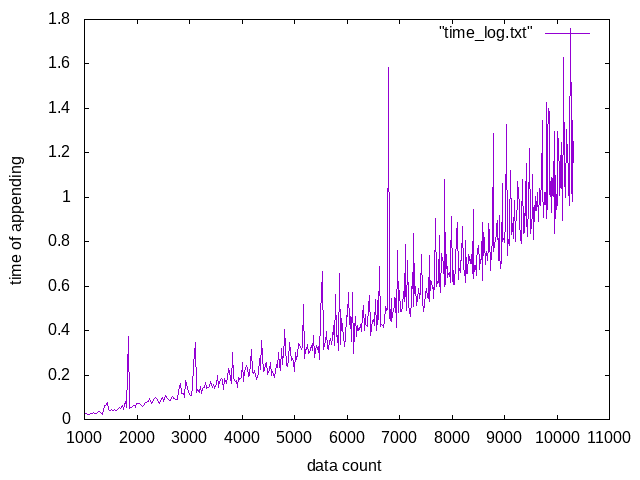
\includegraphics[scale=0.5]{plot3+-?!} 
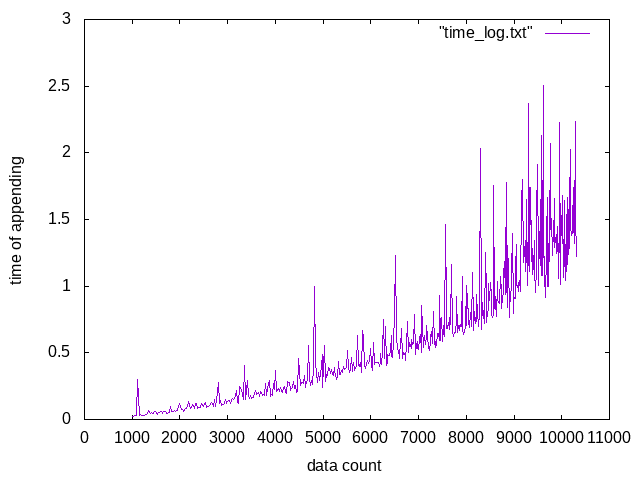
\includegraphics[scale=0.5]{plot5+-?!} 

Несмотря на то, что изначальный вариант программы имеет лучшие результаты, видно, что ассимптотика у них одинаковая, а из-за шума посторонних процессов компьютера сложно
наверняка определить, какой из вариантов лучше. В первом случае сложность загрузки $nlog_2 n$, так как мы вытаскиваем из файла по одному элементу ($O(n)$), и вставляем в дерево
за $log_2 n$. Во втором случае мы встречаемся с элементом только один раз, вставляем и больше к нему не возвращаемся, из чего следует сложность ($O(n)$). Однако как мы убедились
на прошлых графиках, вставка на таком количестве элементов производится почти за константное время, поэтому графики выходят с практически одинаковой ассимптотикой. Почему не 
линейный вид графика? Потому что считается время выполнения всей программы, а значит чем больше команд подается, тем больше сохранений и загрузок будут появляться в 
разных местах теста, когда в дереве то 10 элементов, то 10000. Точный расчет сложности от таких случайных тестов должен включать теорию вероятностей, поэтому на данный момент
остается для меня нерешаемой задачей.

Утилита Perf предоставляет инструмент анализа производительности в Linux посредством счетчиков. К сожалению, документация этой утилиты крайне сложная и размытая, однако
я попытался чуть-чуть разобраться. Задача, которую я хочу достичь с помощью Perf - узнать распределение нагрузки частей программы на процессор. Что работает медленнее (а значит 
дольше), а что работает хорошо. Первая сложность появилась на этапе запуска этой утилиты. Выдавалась ошибка об отказе доступа, которая решалась запуском с sudo. Разобравшись
со множеством непонятного синтаксиса команд, я смог запустить в итоге трассировку именной моей пользовательской программы, а не всех процессов компьютера.

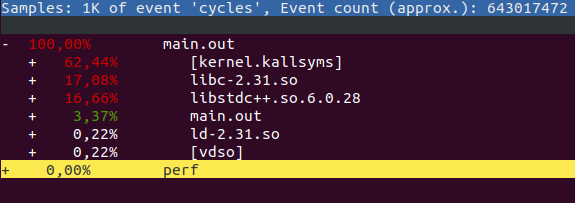
\includegraphics[width=\textwidth]{../scrins/02}

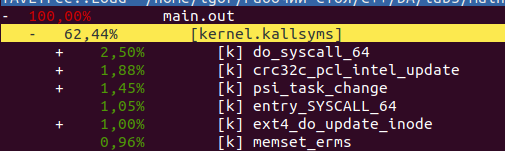
\includegraphics[width=\textwidth]{../scrins/05} 

Из первых двух скриншотов мы видим, что большая часть нагрузок пала на системные вызовы ядра, что не удивительно. 
В основном все они внутри распределены равномерно и каждому уходит не более 2\%, кроме do\_syscall\_64. 

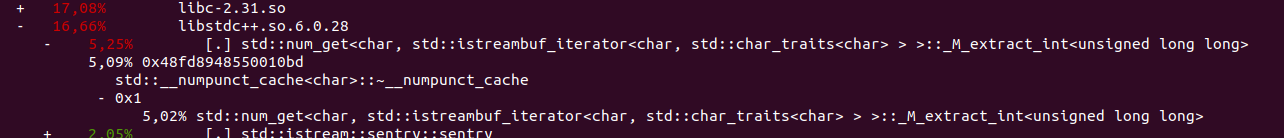
\includegraphics[width=\textwidth]{../scrins/06} 

Из библиотек std больше всего уходит нагрузка на вызов функции num\_get, связанная с вводом и выводом, записью и чтением чисел, так как изначально они представляются в виде символов. То есть это своего рода парсер, а так как ввода и вывода, записи и чтения при командах загрузки и сохранения дерева много, то такой расход ресурсов вполне объясняется.

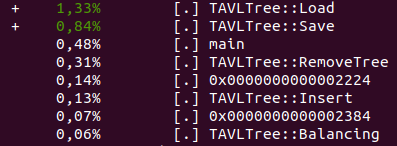
\includegraphics[width=\textwidth]{../scrins/07} 

Как и предполагалось, функция Load использует больше всего ресурсов, нежели функции вставки, удаления, перебалансировки и даже сохранения в файл.

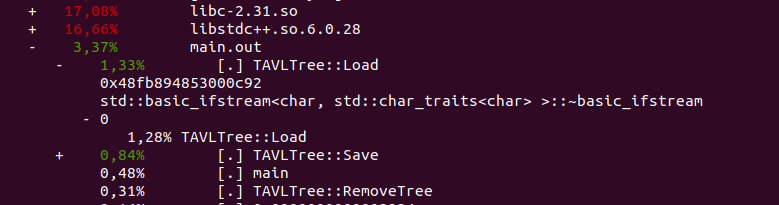
\includegraphics[width=\textwidth]{../scrins/04}

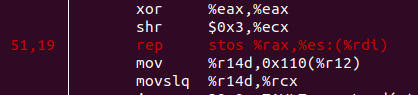
\includegraphics[width=\textwidth]{../scrins/03} 

И если мы пойдем глубже, то увидим, что у нас слишком часто используется ассемблерная команда REP повторения строковой операции, а именно REP STOS - заполнение блока по адресу
содержимым. Странным оказалось то, что я не увидел нагрузку на сравнение строк, хотя казалось бы, что это занимает достаточное количества времени, и по-хорошему было бы их
хэшировать, чтобы добиться оптимизации кода.

Привести интересные проверки с valgrind'ом я не смогу, так как все утечки памяти были устранены раннее. Класс NMystd::string, написанный для второй лабораторной работы по
условию задачи имеет ограничение на 256 символов, поэтому я не делал динамическое выделение памяти для этого типа и никаких утечек там быть не могло, а AVL-дерево достаточно
простое и утечки памяти, к примеру, при удалении узла было легко отследить и устранить. 

\pagebreak
